\section{系统实现}

针对以上设计,我们实现了 AquaFS 文件系统。
AquaFS 文件系统的实现基于 ZenFS,我们在 ZenFS 的基础上进行了修改和优化,使其支持 RAID 等功能。

在初赛阶段,由于人手不足等问题,我们优先实现 AquaFS 文件系统的以下几个部分:

\begin{enumerate}
  \item AquaFS 文件系统的 RAID 实现
  \item AquaFS 的 IO 加速实现
  \item AquaFS 文件系统的智能调参模块实现
  \item AquaFS 文件系统的功能和性能测试
\end{enumerate}

在复赛阶段,我们将继续完善 AquaFS 文件系统其余模块的实现,包括智能数据分类、通用 VFS 文件系统接口等。

\subsection{AquaFS 文件系统的 RAID 实现}

当前 AquaFS 的 RAID 实现主要分为两种:全盘 RAID 和分区 RAID。这两种 RAID 实现的区别在于,全盘 RAID 的 RAID 单位是磁盘,而分区 RAID 的 RAID 单位是 Zone。

\subsubsection{全盘 RAID 的实现}

在传统的 RAID 实现中,基本都是以磁盘为单位进行数据 RAID 逻辑。以磁盘为单位的 RAID 能够充分运用各个磁盘的数据吞吐,并基于 Linux 的块设备等抽象层提供软件上的 RAID 功能。我们也首先实现了全盘 RAID 的功能,能够将多个 ZNS 配置为 RAID 0、RAID 1 模式。

由于 ZenFS 是一个没有一般 POSIX 接口的文件系统,其仅向上服务于 RocksDB,所以我们并不能简单地使用 Linux 上常用的磁盘软件 RAID 来实现 ZNS 的 RAID 功能。更何况,ZNS 并不是 Linux 兼容的块设备,内核中并没有对 ZNS 的 RAID 支持。经过调研和评估,我们认为在 Linux Kernel 内实现对 ZNS 的 RAID 支持并不现实。于是,我们需要在 ZenFS 的基础上实现 RAID 功能。

ZenFS 的数据读写将会经过以下几个层次:

\begin{enumerate}
  \item RocksDB 的 SSTable
  \item RocksDB 的 MemTable
  \item RocksDB 的 WAL
  \item RocksDB 的 FileSystem
  \item ZenFS 的 ZoneFile
  \item ZenFS 的 ZoneExtent
  \item ZenFS 的 Record
  \item ZenFS 的 ZonedBlockDeviceBackend
  \item libzbd 的 ZbdlibBackend
  \item Linux Kernel 相关系统调用
\end{enumerate}

其中,RocksDB 的 SSTable、MemTable、WAL、FileSystem 都是 RocksDB 的内部实现,ZenFS 的 ZoneFile、ZoneExtent、Record、ZonedBlockDeviceBackend 都是 ZenFS 的内部实现,libzbd 的 ZbdlibBackend 是 ZenFS 内对 libzbd 的接口适配,Linux Kernel 相关系统调用是 libzbd 作为用户态程序调用 Linux Kernel 内的设备驱动程序的接口,最终还是会通过 Linux 的系统调用来实现数据的传输。

ZenFS 和 RocksDB 还支持了另一种数据读写方式,通过 ZoneFS 将 ZNS 中的 Zones 以文件映射到文件系统中,然后通过文件系统的接口来读写数据。这种方式的数据读写流程如下:

\begin{enumerate}
  \item RocksDB 的 SSTable
  \item RocksDB 的 MemTable
  \item RocksDB 的 WAL
  \item RocksDB 的 FileSystem
  \item ZenFS 的 ZoneFile
  \item ZenFS 的 ZoneExtent
  \item ZenFS 的 Record
  \item ZenFS 的 ZonedBlockDeviceBackend
  \item ZoneFS 的 ZoneFSBackend
  \item Linux Kernel VFS 接口
\end{enumerate}

虽然这种方式通过 ZoneFS 将 ZNS 中的 Zones 以文件映射到文件系统中,但是 ZoneFS 并不是一个通用的文件系统,它仅仅是一个将 ZNS 中的 Zones 以文件的形式映射到文件系统中的文件系统。ZoneFS 并不支持文件的创建、删除、重命名等操作,文件的读写操作也支持不完全,而且还会引入更多的存储 IO 栈,所以我们并没有选择通过 ZoneFS 来实现 ZNS 的 RAID 功能。

我们选择在 ZenFS 的 ZonedBlockDeviceBackend 层实现 ZNS 的 RAID 功能。ZonedBlockDeviceBackend 层是 ZenFS 中管理数据后端的层,它是 ZenFS 与 libzbd 或 ZoneFS 之间的接口层,负责将 ZenFS 的数据读写请求转换为 libzbd 或 ZoneFS 的数据读写请求。

我们通过继承 ZonedBlockDeviceBackend 来实现 ZenFS 内的数据 RAID 功能。ZonedBlockDeviceBackend 的继承类图如图 \ref{raid-layers} 所示。

\begin{figure}[htbp]
  \centering
  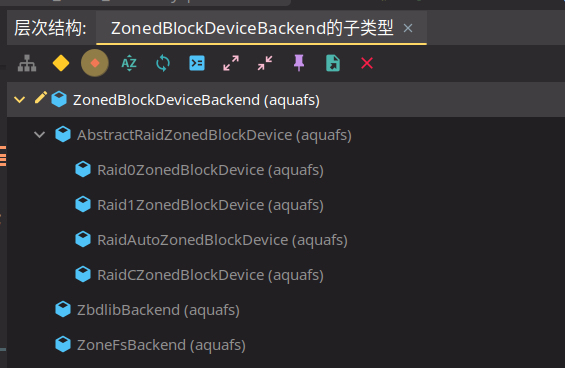
\includegraphics[width=0.85\textwidth]{fig/raid-layers}
  \caption{ ZonedBlockDeviceBackend 继承类图 }
  \label{raid-layers}
\end{figure}

AbstractRaidZonedBlockDevice 下的 Raid0ZonedBlockDevice、Raid1ZonedBlockDevice 和 RaidCZonedBlockDevice 即为全盘 RAID 的实现。其中,Raid0ZonedBlockDevice 实现了 RAID 0 的功能,Raid1ZonedBlockDevice 实现了 RAID 1 的功能,RaidCZonedBlockDevice 实现了 RAID C 的功能。

RAID C 是我们自定义的一种简单 RAID 格式,它通过 Zones 的合并来实现简单的数据拼合逻辑,即将多个 Zone 合并为一个 Zone,然后将数据写入到合并后的 Zone 中。RAID C 的实现如图 \ref{raid-c} 所示。

\begin{figure}[htbp]
  \centering
  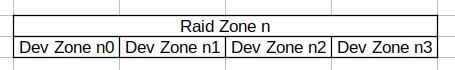
\includegraphics[width=0.85\textwidth]{fig/raid-c}
  \caption{ 全盘 RAID 的数据排布 }
  \label{raid-c}
\end{figure}

此时多个($m$个)设备上实际存在的 Zones 合并为一个大的逻辑 Raid Zone,数据将会按顺序依次写入 Dev Zone $n_{i}$($0 \le i < m$)。此 RAID C 模式存在的意义是,形成一个简单的 Zone 合并逻辑,便于后续开发应用。其中,Dev Zone $n_i$ 分别为来自第 $i$ 个设备的第 $n$ 个 Zone。

RAID 0 和 RAID 1 的实现与传统的 RAID 0 和 RAID 1 的实现类似,RAID 0 将数据分散写入多个设备中,RAID 1 将数据写入多个设备中的一个。RAID 0 和 RAID 1 的实现中的数据排布与 RAID C (图 \ref{raid-c})基本一致。

RAID 0 在写入时,将会将数据分散写入多个设备中。类似于传统块设备的 Block Size,ZNS 也是有最小写入单位的,也是 Block Size。RAID 0 在读写时,可以将读写请求分割为不同的 Block Size 的读写请求,然后对这些请求重新合并排序,再调用底层的读写接口。

以 RAID 0 读为例,其未经 IO 优化的读流程如下所示:

\begin{lstlisting}
int Raid0ZonedBlockDevice::Read(char *buf, int size, uint64_t pos,
                                bool direct) {
#ifndef AQUAFS_RAID_URING
  // split read range as blocks
  int sz_read = 0;
  int r;
  while (size > 0) {
    auto req_size =
        std::min(size, static_cast<int>(GetBlockSize() - pos % GetBlockSize()));
    r = devices_[get_idx_dev(pos)]->Read(buf, req_size, req_pos(pos), direct);
    if (r > 0) {
      size -= r;
      sz_read += r;
      buf += r;
      pos += r;
    } else {
      return r;
    }
  }
  return sz_read;
#else
  // ...
#endif
}
\end{lstlisting}

代码逻辑主要为,每次请求最多读取一个 Block Size 的数据,然后将读取的数据拼接到 buf 中,直到读取完毕。其中需要多次重复计算数据分块的设备位置和块位置,于是这里使用了 get\_idx\_dev 和 req\_pos 函数来快速计算设备位置和块位置。这些函数被实现在 AbstractRaidZonedBlockDevice 层,以便其子类可以快速调用其逻辑。

在上述代码中,我们将读请求分割为不同的 Block Size 的读请求,然后调用底层的读写接口。这样做的好处是,可以将读请求分散到多个设备中,从而提高读性能。不过,上述代码中其实并没有体现 RAID 0 的多设备读优化,还是单线程读取。我们在后文中实现了基于 uring 的多设备并行读优化。

\subsubsection{智能分区 RAID 的实现}

分区 RAID 的实现与全盘 RAID 的实现类似,但是我们在逻辑 Raid Zone 和实际设备 Zone 之间加上了一层基于 Zones 的映射。这些映射是通过 ZenFS 的 Record 写入 MetaZones 内的,将在每次文件系统加载的时候逐步读取加载映射逻辑。

加上这一层映射之后,分区 RAID 的数据排布逻辑可能如图 \ref{raid-a} 所示。

\begin{figure}[htbp]
  \centering
  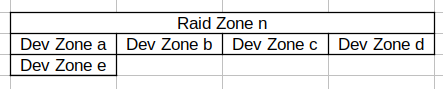
\includegraphics[width=0.85\textwidth]{fig/raid-a}
  \caption{ 分区 RAID 的数据排布 }
  \label{raid-a}
\end{figure}

Zone Raid $n$ 为向上层暴露出的可读写数据 Zone 区域,而其中可以存在多种不同的 RAID 逻辑或映射类型。

在示例图 \ref{raid-a} 中,Dev Zone $x$ 表示来自不同或相同设备的设备上物理存在的 Zone。
如果这个 Raid Zone 被配置为 RAID 1,则 Dev Zone $a$ 和 Dev Zone $e$ 将同时以 RAID 1 数据冗余方式为 Raid Zone $n$ 的前四分之一数据提供服务,其他 Dev Zones 由于没有映射,将回退到 RAID C 逻辑提供数据存储服务。若这个 Raid Zone 被配置为 RAID 0,则 Dev Zone $a$ 和 Dev Zone $e$ 将同时以 RAID 0 数据分散方式为 Raid Zone $n$ 的前四分之一数据提供服务,其他 Dev Zones 由于没有映射,将回退到 RAID C 逻辑提供数据存储服务。

实际代码实现上,除了上述映射逻辑处理,还有许多细节需要考虑。

首先是跨 Zones 读写问题。由于我们添加的映射逻辑,使得我们的数据排布不再是连续的,而是以 Zones 为单位分散的。这就导致了我们的读写请求可能会跨越多个 Zone。这就需要我们在读写时,需要将读写请求分割为不同的 Block Size 的读写请求,然后可能对这些请求重新合并排序,再调用底层的读写接口。

在读或写代码中,通过数据段分割并递归调用自身的方式实现跨 Zones 读写的请求分割:

\begin{lstlisting}
  if (static_cast<decltype(zone_sz_)>(size) > zone_sz_) {
    // may cross raid zone, split read range as zones
    int sz_read = 0;
    int r;
    while (size > 0) {
      auto req_size =
          std::min(size, static_cast<int>(zone_sz_ - pos % zone_sz_));
      r = Read(buf, req_size, pos, direct);
      if (r > 0) {
        buf += r;
        pos += r;
        sz_read += r;
        size -= r;
      } else {
        return r;
      }
    }
    // flush_zone_info();
    return sz_read;
  } else {
    // ...
\end{lstlisting}

其次是数据后端问题。由于我们是基于 ZonedBlockDeviceBackend 来实现的,而 ZonedBlockDeviceBackend 有多种子类,可以是 libzbd、ZoneFS 甚至是原来实现的全盘 RAID。
为了进一步简化 IO 调用栈,我们在实现分区 RAID 时,假定数据后端都是 libzbd 提供的数据读写。这在之后可以进一步优化,以支持更多的数据后端,提升 RAID 逻辑的灵活性,如添加 ZoneFS 支持、添加 SPDK 等 Kernel bypass 方案支持等。

除此以外,还需要考虑对 ZenFS 的兼容性问题。ZenFS 在加载的过程中,会对固定的 MetaZones 进行扫描,通过 Magic Number 查找到 Meta Zones 中的可用的超级块,并选择最新的超级块进行文件系统初始化。为了兼容 ZenFS 的 Meta Data 管理逻辑,我们不能改变 MetaZones 的排布,也不能改变超级块的存储逻辑。因此,我们在实现分区 RAID 时,需要保证 MetaZones 的排布不变,超级块的存储逻辑不变,以及超级块的存储位置不变。所以,我们在实现分区 RAID 时,将 MetaZones 的排布和超级块的存储位置都固定在了第一个设备上,进行映射的连续逻辑预分配,这样就可以保证 ZenFS 的兼容性,使得 ZenFS 在加载分区 RAID 时,可以正常加载。

在创建或读取文件系统时的预分配映射:

\begin{lstlisting}
  // create temporal device map: AQUAFS_META_ZONES in the first device is used
  // as meta zones, and marked as RAID_NONE; others are marked as RAID_C
  for (idx_t idx = 0; idx < AQUAFS_META_ZONES; idx++) {
    for (size_t i = 0; i < nr_dev(); i++)
      allocator.addMapping(idx * nr_dev() + i, 0, idx * nr_dev() + i);
    allocator.setMappingMode(idx, RaidMode::RAID_NONE);
  }
\end{lstlisting}

为了管理分区之间的映射关系,我们通过组合的方式实现了一个分区分配器 ZoneRaidAllocator。其可以管理分区的映射关系,以及分区的 RAID 逻辑。其主要接口如下:

\begin{lstlisting}
  Status addMapping(idx_t logical_raid_zone_sub_idx, idx_t physical_device_idx,
                    idx_t physical_zone_idx);
  void setMappingMode(idx_t logical_raid_zone_idx, RaidModeItem mode);
  void setMappingMode(idx_t logical_raid_zone_idx, RaidMode mode);

  int getFreeDeviceZone(idx_t device);
  int getFreeZoneDevice(idx_t device_zone);
  Status createMapping(idx_t logical_raid_zone_idx);
  Status createMappingTwice(idx_t logical_raid_zone_idx);
  Status createOneMappingAt(idx_t logical_raid_zone_sub_idx, idx_t device,
                            idx_t &zone);
  void setOffline(idx_t device, idx_t zone);
\end{lstlisting}

其可以提供映射关系的查询、增加、删除、修改等功能,以及提供 Raid Zone 所分配的 RAID 逻辑的查询、增加、删除、修改等功能。

同时,它还提供了 setOffline 功能,可以在发现设备故障时,将故障设备的所有分区设置为 Offline 状态,以便后续的故障处理。

\subsubsection{分区 RAID 故障处理}

在分区 RAID 故障处理方面,我们实现了基于分区 RAID 的故障处理方案。其主要思路是,当发现设备故障时,将故障设备的所有分区设置为 Offline 状态,然后将所有的分区重新映射到其他设备上,以保证数据的可用性。

由于在调研中我们发现,Nand Flash 向上提供的数据一般含有 ECC 校验和纠错,且 ZenFS 中的 Record 也有 CRC 校验和,所以我们认为在数据传输过程中,较少比特数据的完整性是可以保证的。所以,我们在实现分区 RAID 故障处理时,仅考虑大块数据的完整性恢复,而不考虑小块数据的完整性。

\begin{lstlisting}
  // 在数据操作函数中
  if (r < 0) {
    auto status = ScanAndHandleOffline();
    if (status.ok()) {
      // retry this read
      return Read(buf, size, pos, direct);
    } else {
      Error(logger_, "failed to restore data: %s", status.getState());
      return r;
    }
  }
\end{lstlisting}

ScanAndHandleOffline 函数将扫描当前所有盘的数据状态,如果发现有盘处于 Offline 状态,则将所有的分区重新映射到其他设备上,并根据 RAID 逻辑进行数据恢复。

当前由于仅实现了 RAID 0 和 RAID 1 的数据逻辑,所以暂时仅支持 RAID 1 分区的数据恢复。当发现 RAID 1 分区的数据不一致时,将重新选择一个 Dev Zone,将数据恢复到新的 Dev Zone 上。

当前的故障处理逻辑还相对比较简单,在复赛中实现更多 RAID 逻辑后,将进一步改进此部分的故障处理逻辑,如增加 RAID 5 的故障处理逻辑、增加故障恢复的并发度等。

\subsection{AquaFS 的 IO 加速实现}

在上文中,我们已经介绍了 AquaFS 的 RAID 方案,但是由于是比较初级的版本,很多代码并没有进行并行优化,仍然是单线程的。所以,我们在实现 IO 加速方面,主要是对 RAID 下的 IO 操作进行并行优化。

在我们实现之前,ZenFS 的 IO 优化主要是从 RocksDB 中继承而来。RocksDB 中可以使用 Direct IO 来读写文件,以避免数据在用户态和内核态之间的拷贝。其 Direct IO 优化既可以用于 RocksDB 的 PosixFileSystem 常规文件系统后端,也可以用于 RocksDB 的 ZenFS 文件系统后端。

Direct IO 主要的优化逻辑是,将用户态的数据缓冲区直接映射到内核态的页缓存中,从而避免了数据在用户态和内核态之间的拷贝。通过 Direct IO 打开的设备,从设备中获得的数据将直接写入在用户态的数据缓冲区中,而不是先写入内核态的页缓存中,从而减少了一次数据拷贝。

Direct IO 的使用也非常简单,只需要在打开文件时,将 O\_DIRECT 标志传入即可。但是,由于 Direct IO 的使用需要满足一些条件,如文件的偏移量和长度需要是当前系统内存页大小的整数倍,所以在使用 Direct IO 时,需要对文件的偏移量和长度进行调整。

我们发现,在我们的加速方案中,Direct IO 可以与更多的 IO 加速方案并存。如在我们的加速方案中,我们可以使用 io\_uring 来加速 IO 操作,而 io\_uring 也可以与 Direct IO 并存。

在加速方案选择上,我们选择了 io\_uring 方案。当前 Linux 系统上有许多 IO 加速方案,如 AIO、io\_uring、libaio 等,如图 \ref{io-speedup} 所示。

\begin{figure}[htbp]
  \centering
  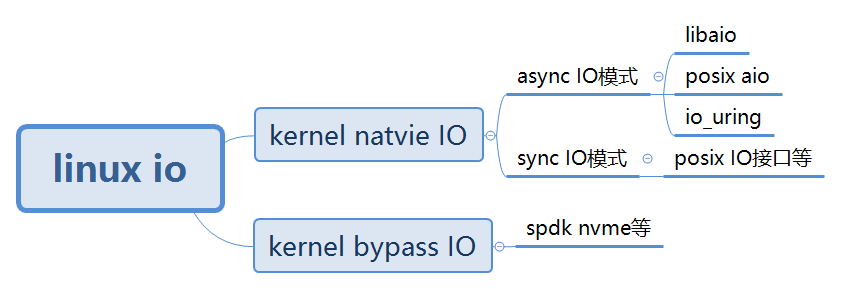
\includegraphics[width=0.7\textwidth]{fig/io-speedup}
  \caption{IO 加速方案}
  \label{io-speedup}
\end{figure}

io\_uring 是 kernel natvie aio 的一种,它是 Linux Kernel 5.1 版本加入一个特性。io\_uring 围绕高效进行设计,其设计了一对共享的 ring buffer 用于应用和内核之间的通信,通过该设计实现了如下的三个好处:

\begin{enumerate}
  \item 避免在提交和完成事件中存在内存拷贝;
  \item 避免了 libaio 中在提交和完成任务的时候系统调用过程;
  \item 该队列采用了无锁的访问模式,通过内存屏障减少了竞争。
\end{enumerate}

io\_uring 的使用也非常简单,只需要提交 SQE 到 ring buffer 中,然后等待 CQE 即可。
由于其简单使用、高效的设计,我们选择了 io\_uring 作为我们的 IO 加速方案。

其实 io\_uring 在 RocksDB 的 PosixFileSystem 文件系统后端中已经有可选的实现,但是它并没有被实现到 ZenFS 后端中,ZenFS 的数据读写还是只能使用 Direct IO 进行优化。于是,我们在 ZenFS 的文件系统后端中实现了 io\_uring 的优化,从而进一步加速了 ZenFS 的 IO 操作。

为了进一步增大 IO 加速的效果,我们还实现了 IO 操作的批处理。在原版 ZenFS 中,IO 操作是以单个系统调用的形式进行的,即每次 IO 操作都是单个请求。但是如果将多个 IO 操作打包成一个批处理请求,可以进一步提高 IO 操作的效率,尤其是单 IO 请求的效率。

为了实现 IO 操作的批处理,我们在 AquaZFS 的文件系统后端中实现了 IO 请求的分割和合并,并将请求全部打包成一个批处理请求,然后一次性提交给 io\_uring,从而实现了 IO 操作的批处理。

除了上述优化处理,我们还使用 C++ 20 的协程特性,进一步增大了代码的并行性。
在调研过程中,我们找到了一个 C++ 实现的 io\_uring 绑定库,其向外提供了协程接口,可以在协程中使用 io\_uring。我们将其移植到了 AquaFS 中,从而实现了在协程中使用 io\_uring。

有关逻辑可以在数据操作相关的函数中找到,如下以读数据函数 Read 为例:

\begin{lstlisting}
  using req_item_t = std::tuple<int, char *, uint64_t, off_t>;
  std::vector<req_item_t> requests;
  std::vector<ZbdlibBackend *> bes(nr_dev());
  for (decltype(nr_dev()) i = 0; i < nr_dev(); i++) {
#ifdef ROCKSDB_USE_RTTI
    bes[i] = dynamic_cast<ZbdlibBackend *>(devices_[i].get());
    assert(bes[i] != nullptr);
#else
    bes[i] = (ZbdlibBackend *)(devices_[i].get());
#endif
  }
  while (size > 0) {
    // ...
    requests.emplace_back(fd, buf, req_size, mapped_pos);
    // ...
  }
\end{lstlisting}

如上所示,我们首先将 IO 请求分割成多个小的 IO 请求,将这些请求收集到 std::vector 中。
由于 ZNS 支持随机读,所以可直接将 IO 请求加入到 std::vector 中,而无需考虑 IO 请求的顺序。

收集到 IO 读请求后,我们将这些请求打包成一个批处理请求,然后一次性提交给 io\_uring,如下所示:

\begin{lstlisting}
  uio::io_service service;
  // ...
  service.run([&]() -> uio::task<> {
    std::vector<uio::task<int>> futures;
    for (auto &&req : requests) {
      uint8_t flags = 0;
      // read do not need order
      // if (req != *req_list.second.cend()) flags |= IOSQE_IO_LINK;
      futures.emplace_back(service.read(std::get<0>(req), std::get<1>(req),
                                        std::get<2>(req), std::get<3>(req),
                                        flags) |
                           uio::panic_on_err("failed to read!", true));
    }
    for (auto &&fut : futures) co_await fut;
  }());
\end{lstlisting}

在作为举例的 Read 函数中,我们首先创建了一个 service 对象,然后使用 run 方法启动协程,在协程中逐个将请求提交到 SQE 中,然后等待所有的 CQE 即可。这里的 flags 参数用于指定 IO 请求的属性,如 IOSQE\_IO\_LINK 表示该 IO 请求是一个批处理请求中的一部分。由于我们的 IO 请求是无序的,所以我们不需要使用 IOSQE\_IO\_LINK。

在写操作相关的函数中,相比于读操作,还需要基于 ZNS 的顺序写特性考虑更多的因素,如下所示:

\begin{lstlisting}
  using req_item_t = std::tuple<char *, uint64_t, off_t>;
  // <dev, zone> -> vec<ordered req>
  std::map<std::pair<int, idx_t>, std::vector<req_item_t>> requests;
\end{lstlisting}

我们首先将 IO 请求按照设备和 Zone 序号进行分组,然后将每个 Zone 内的 IO 请求按照顺序进行排序,最后将这些请求收集到 std::vector 中。而在提交 IO 请求时,我们需要将这些请求按照顺序依次提交。

总之,我们在 AquaFS 中实现了 io\_uring 和 C++20 协程 的优化,从而进一步加速了 AquaFS 的 IO 操作。

\subsection{AquaFS 文件系统的智能调参模块实现}

智能调参模块方面,实现了基于方差的重要参数选择方案和基于高斯过程回归的参数调整方案。

\begin{figure}[htbp]
  \centering
  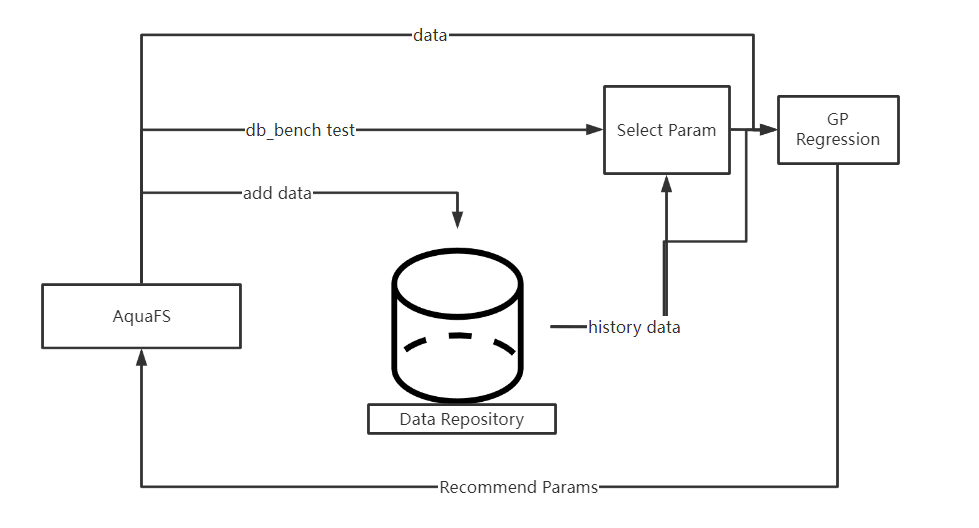
\includegraphics[width=0.7\textwidth]{fig/aquaturnner}
  \caption{AquaTurnner 智能调参模块}
  \label{aquaturnner}
\end{figure}

如图 \ref{aquaturnner} 所示,AquaTurnner 智能调参模块主要由三部分组成,被调对象,本文中是AquaFS,历史数据存储仓库,以及调参事务组成,调参事务又包括选择参数选择模块和高斯过程回归调整参数模块。

首先,AquaFS需要预热地运行,收集到不同参数配置下的目标指标,本文中使用的是吞吐量指标,将对应的参数配置和目标指标值存入数据仓库中。在初次预热之后,后续不须要预热,除非加入了新的参数指标。

考虑到AquaFS作为RocksDB的插件存在,在本文中使用RocksDB的测试脚本db\_bench来测试系统的吞吐量,采用prometheus作为收集数据的工具。在这个测试中,用收集到的目标指标值和配置参数值,配合历史数据仓库中的数据,来进行参数选择和高斯过程回归。参数选择模块根据方差指标选择最重要的几个参数,高斯过程回归用重要的参数和目标指标值进行拟合以及回归。

首先对于最重要的参数,由方差计算的最大值对应的参数得到:

\begin{equation}
  \label{eq:var}
  \begin{aligned}
    Var(S)=\frac{1}{\lvert S\rvert}\sum_{i=1}^{\lvert S\rvert}(y_i-\mu)^2 \\
    PI(P)=Var(S)-\sum_{i=1}^{N}\frac{S_{P=P_i}}{S}Var(S_{p=p_i})
  \end{aligned}
\end{equation}

这里的 $y_i$ 是样本中的目标值,$\mu$ 是样本目标值均值,$PI$ 系数是基于方差来计算的,即固定某一个参数的值,根据参数的值划分集合,在每个集合中求出集合中目标值的对应方差,再用初始方差 $Var(S)$ 减去这个和,这个 $PI$ 系数越大说明原来的这个参数的影响越大,因为在同一个值的情况下,集合内方差的和很小。

其次由 $CPI$ 指标来选择剩余重要参数:

\begin{equation}
  \label{eq:cpi}
  \begin{aligned}
    CPI(Q|P=p) = Var(S_{P=p})-\sum_{j=1}^{m}\frac{S_{Q=Q_{w_j},P=p}}{S_{P=p}}Var(S_{Q=q_i|P=p})\\
    CPI(Q|P=p) = \max_{1\le i\le n}CPI(Q|P=p_i)
  \end{aligned}
\end{equation}

基于方差的重要参数选择算法如算法 \ref{alg:aquaturnner_select} 所示。

\begin{algorithm}[htb]
  \caption{ AquaTuner参数选择算法 }
  \label{alg:aquaturnner_select}
  \begin{algorithmic}[1]
    \Require
      adjust\_param\_num, db\_bench\_data, data in repository
    \Ensure
      important\_params
    \State important\_params = []
    \State Select the most important param by $PI(param)$, add to important\_params;
    \State For $i$ in adjust\_param\_num $–$ $1$:
    \State \qquad Compute $CPI$ for each param that not in important\_params;
    \State \qquad Select the largest $CPI$’s corresonding params to important params; \\
    \Return important\_params
  \end{algorithmic}
\end{algorithm}

对于连续参数,AquaTuner对于参数指标在参数范围内给出合适的推荐参数值,该合适参数值是在拟合的高斯过程模型曲线上,根据在最优配置参数附近做抖动获得,也即尝试最优配置参数点附近的参数值看目标指标是否有所提升,对于离散参数,AquaTunar尝试匹配最优目标指标值对应的配置参数的离散值。

AquaTuner的运行算法流程如算法 \ref{alg:aquaturnner_trunning} 所示。

\begin{algorithm}[htb]
  \caption{ AquaTuner参数调优算法 }
  \label{alg:aquaturnner_trunning}
  \begin{algorithmic}[2]
    \Require
      adjust\_param\_num
    \Ensure
      recommend\_param
    \State data repository <- warm up system and collect data;
    \State start db\_bench;
    \State db\_bench\_data = collect data from db\_bench;
    \State add db\_bench\_data to data repository;
    \State important\_params = Select\_Param(adjust\_param\_num ,db\_bench\_data, data in repository);
    \State GP\_model = GP\_regression(important\_params, eb\_bench\_data, data in repository);
    \State recommend\_param = [];
    \State For param in  history\_best\_params and important params:
    \State \qquad If param is continuous:
    \State \qquad \qquad Try values near the past value, add to recommend\_param;
    \State \qquad Else if param is discrete:
    \State \qquad \qquad Try values in best params,add to recommend\_param;
    \State Target = GP\_model.predict(recommend\_param);
    \State If Target is better:
    \State \qquad \Return recommend\_param;
    \State \Return history\_best\_param;
  \end{algorithmic}
\end{algorithm}
